\section{Hosting serwera}
\label{przygotowania:hosting}
Zanim przystąpimy do implementacji aplikacji serwerowej chciałem zdecydować o sposobie jej udostępnienia publicznie.
Połączenie do serwera lokalnego hostowanego w tej samej sieci lokalnej, w której znajduje się telefon użytkownika, jest możliwe, ale wymagałoby to wielu dodatkowych zmian.
W przypadku łączenia do serwera działającego na localhost, telefon musiałby być podłączony do tej samej sieci lokalnej, co serwer i aplikacja kliencka musiałaby mieć wyłączone zabezpieczenia, które blokują połączenia z zewnątrz.
Niestety jest to kompletnie zły sposób interakcji z serwerem, ponieważ nie jest to skalowalne i nie jest to bezpieczne.
Z tego powodu zdecydowałem się na zbadanie możliwości serwisów hostingowych, które umożliwiają hostowanie aplikacji serwerowych.
Heroku jest jedną z najbardziej popularnych platform do hostowania aplikacji serwerowych.
Pozwala również na odpowiednie skalowanie aplikacji, co jest bardzo ważne w przypadku, gdy aplikacja zyska na popularności.
Dodatkowo platforma oferowała przez długi czas darmowy plan, który pozwalał na hostowanie aplikacji bez ponoszenia kosztów póki nie przekroczy się pewnych limitów.
Byłoby to idealne rozwiązanie dla aplikacji, która nie jest jeszcze w pełni rozwinięta i nie jest jeszcze gotowa na płacenie za hosting.
Niestety heroku zmieniło swoją politykę i obecnie nie oferuje darmowego planu dla aplikacji serwerowych.
\cite{herokuPrice}
W przypadku aplikacji serwerowej planowałem użycie takich technologii jak:
\begin{itemize}
    \item Redis - baza danych NoSQL, która jest wykorzystywana do przechowywania sesji użytkowników.
    \item PostgreSQL - baza danych relacyjna, która jest wykorzystywana do przechowywania danych aplikacji.
    \item Spring Boot - framework do tworzenia aplikacji serwerowych w języku Java.
\end{itemize}

Plany serwisów umożliwiających hostowanie aplikacji serwerowych są ściśle związane z pamięcią RAM, która jest dostępna dla aplikacji.
W przypadku heroku plany są następujące:
\begin{figure}[H]
    \centering
    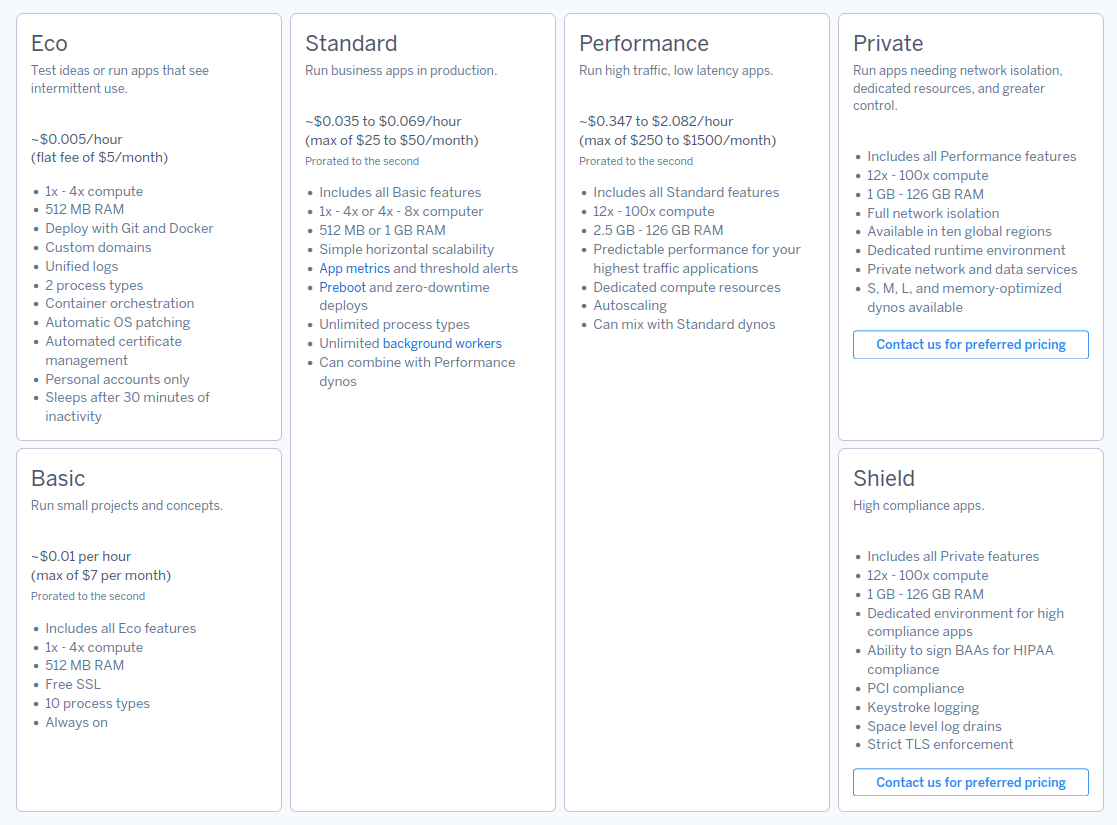
\includegraphics[width=15cm,keepaspectratio]{rysunki/heroku-pricing.png}
    \captionof{figure}{Plan cennikowy Heroku}
    \label{fig:herokuPlans}
\end{figure}

Z tego powodu konieczne było zbadanie aproksymowanej ilości pamięci, która będzie potrzebna dla aplikacji.
Spring Boot używa puli wątków do obsługi zapytań HTTP.
Domyślnie puli wątków jest 200, ale można ją zmienić w pliku konfiguracyjnym aplikacji.
\cite{springBootThreadPool}
Oznacza to, że aplikacja może obsłużyć 200 zapytań jednocześnie, każde kolejne zapytanie będzie czekać na zwolnienie wątku.
Każdy wątek zużywa pewną ilość pamięci RAM, dla ułatwienia obliczeń przyjmijmy, że każdy wątek zużywa 1MB pamięci.
Oznacza to, że dla 200 wątków potrzebujemy 200MB pamięci RAM.
Dodatkowo sama aplikacja zużywa pewną ilość pamięci, która będzie zależeć od ilości zależności, które są używane.
Biorąc pod uwagę również użucie postgreSQL i redis, które również zużywają pewną ilość pamięci, możemy aproksymować, że potrzebujemy około 500MB pamięci RAM.
W takim scenariuszu żaden plan darmowy dostępny na chwilę obecną nie spełniałby naszych wymagań.
Sprawdziłem również inne serwisy hostingowe takie jak:
\begin{itemize}
    \item Fly.io
    \item Netlify
    \item Vercel
\end{itemize}
Niestety żaden z tych serwisów nie oferował darmowego planu dla aplikacji serwerowych.
Dodatkową możliwością byłoby skorzystanie z prywatnego serwera VPS, który oferuje dużo większą elastyczność i możliwości konfiguracji.
Niestety skutkowałoby to koniecznością wykonania dużej ilości dodatkowej pracy, która nie jest związana z tematem pracy.
Z tego powodu zdecydowałem się na skorzystanie z serwisu ngrok, który umożliwia hostowanie aplikacji serwerowych na własnym komputerze.
\cite{ngrok}
Ngrok służy do tunelowania połączeń z zewnątrz do naszego komputera.
Rozwiązanie to pozwala na odpowiednią konfigurację aplikacji serwerowej, która będzie dostępna z zewnątrz.
Ngrok oferuje darmowy plan, który spełnia nasze wymagania.
Dodatkowym atutem jest to, że nie wymaga żadnych ścisłych powiązań z aplikacją serwerową.
Oznacza to, że aplikacja serwerowa nie musi być dostosowana do tego konkretnego serwisu.
Pozwoli to na łatwe przeniesienie aplikacji na inny serwis hostingowy w przyszłości bez konieczności zmian w aplikacji serwerowej.
\clearpage